\section{Further tests}

\subsection{Intel compiled code performances}
Not happy of the previous results, we decided to move from GCC to Intel proprietary compiler, as advised also by the Cineca authorities.
The Intel C++ Compiler 18 is designed to take care of the MIC architecture, using dedicated flags during the compilation process.\par
Using 
\begin{lstlisting}
-AVX512 -parallel
\end{lstlisting}
flags is possible to instruct the compiler to generate vectorized code autonomously. Although there are no guarantees that all loops will be vectorized, leading this solution to be less efficient than an OpenMP implementation, the usage of these flags speeded up our code roughly of a factor two, providing also doubled efficiency with respect to the previous GCC solution, as can be seen comparing figure~\ref{intel:speedup} with~\ref{1287} and figure~\ref{intel:efficiency} with~\ref{1289}.\\~\\

\begin{figure}
\begin{center}
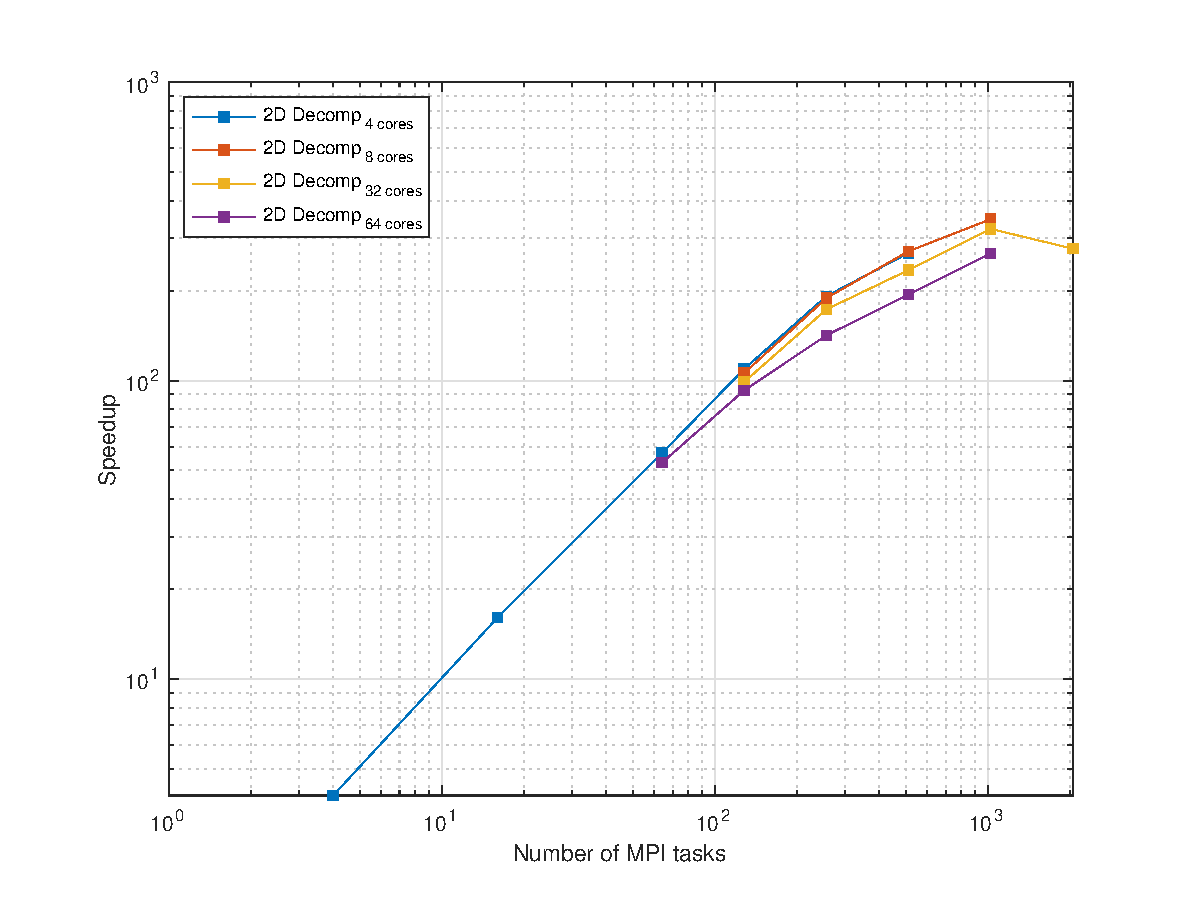
\includegraphics[scale=0.55]{grafici/intel_speedup}
\caption{Speedup using 2D decomposition for $256\times 256\times 512$  simulation with Intel Compiler 18}
\label{intel:speedup}
\end{center}
\end{figure}

\begin{figure}
\begin{center}
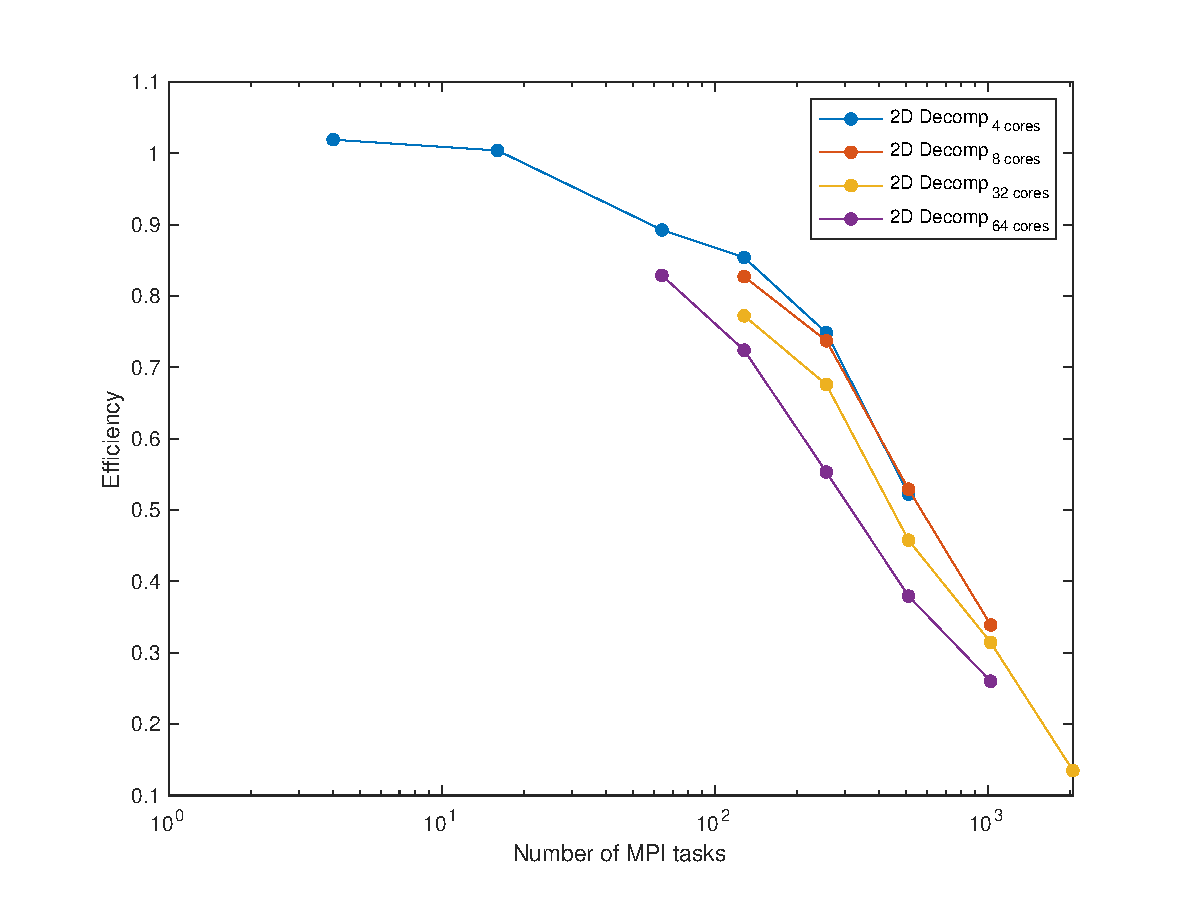
\includegraphics[scale=0.55]{grafici/intel_efficiency}
\caption{Efficiency using 2D decomposition for $256\times 256\times 512$  simulation with Intel Compiler 18}
\label{intel:efficiency}
\end{center}
\end{figure}

As before, the performance peak remains at 1024 simultaneous tasks, however the maximum speedup moved from 178.9, of the 8 cores run using GCC, to 347.1, using the same number of cores with Intel compiler compiled code, with an efficiency not far from the 40\% threshold.
The efficiency gap between the 64 cores runs and the 4 cores ones remains around the 10\%, but the double efficiency with respect to the GCC solution enables the possibility to use 64 cores during production.\\~\\

Next to the already cited flags we used others to refine the auto-vectorization process, in particular the distribution of the MPI tasks among the tiles of the processors, that in this configuration tends to fill adjacent cores with adjacent arrays values, the prefetching level and the mapping of the High Bandwidth Memory, that in this configuration is available as L3 cache memory.
We also moved to a deeper level of optimization and we have disabled fractions in favor to reciprocal multiplications.





\subsection{Performances on GALILeO}